\documentclass[a4paper]{article}
\usepackage[left=0mm,top=5mm,right=0mm,bottom=0mm]{geometry}
\usepackage{tikz}
\usepgflibrary{patterns}
\begin{document}
\thispagestyle{empty}
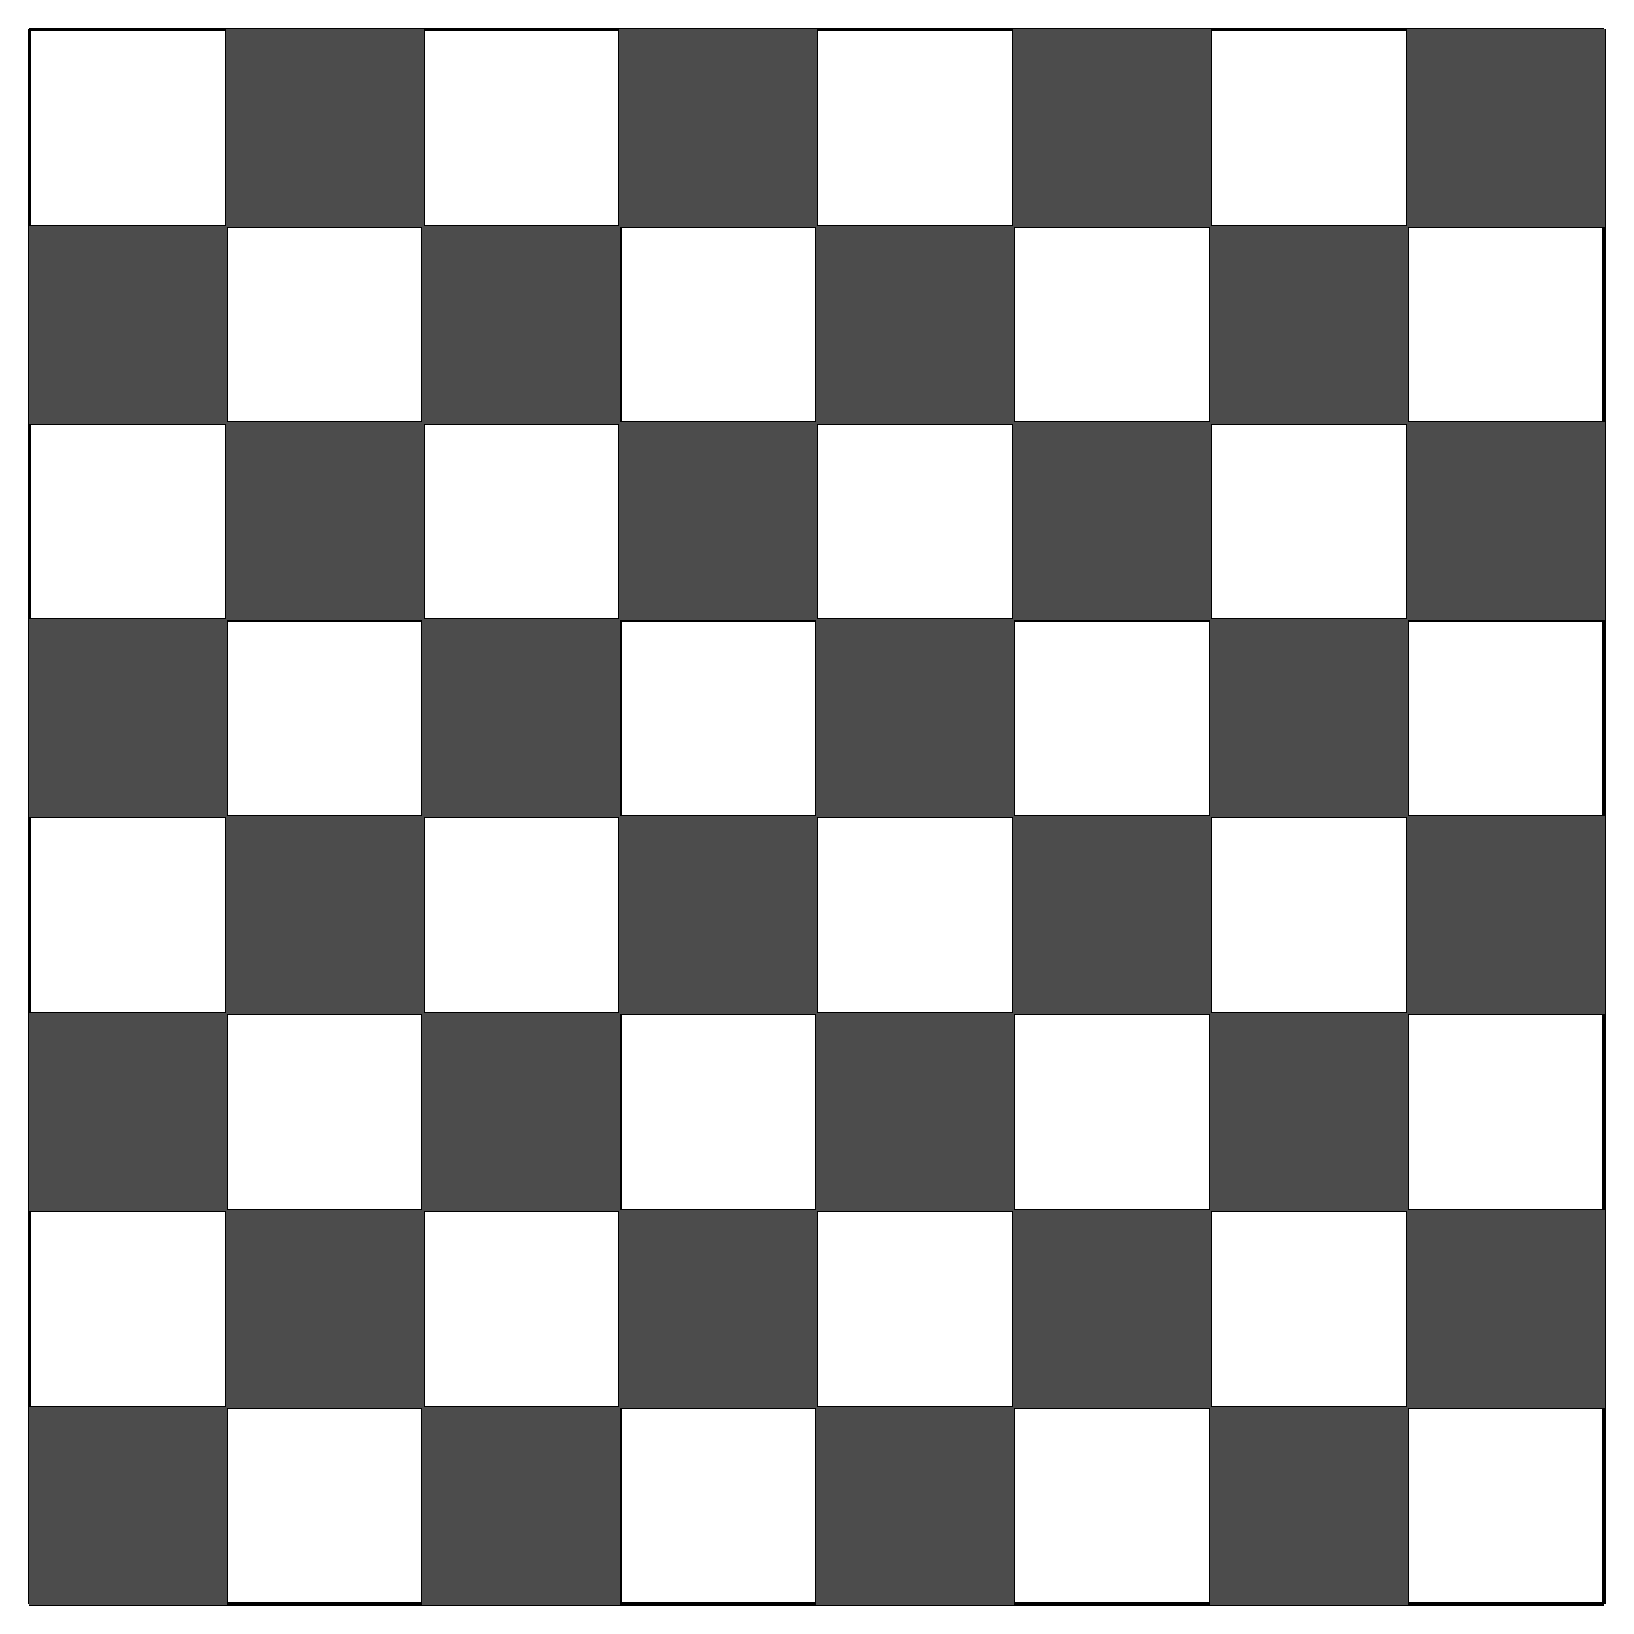
\begin{tikzpicture}
    \draw[step=2.5,very thick] (0,0) grid (20,20);
    \foreach \x in {0,2.5,...,17.5} {
        \foreach \y in {0,2.5,...,17.5} {
            \pgfmathtruncatemacro{\shade}{mod(\x/2.5+\y/2.5,2)}
            \ifnum\shade=0
                \filldraw[black!70] (\x,\y) rectangle (\x+2.5,\y+2.5);
            \fi
        }
    }
\end{tikzpicture}
\end{document}